% Options for packages loaded elsewhere
\PassOptionsToPackage{unicode}{hyperref}
\PassOptionsToPackage{hyphens}{url}
%
\documentclass[
]{article}
\usepackage{amsmath,amssymb}
\usepackage{lmodern}
\usepackage{ifxetex,ifluatex}
\ifnum 0\ifxetex 1\fi\ifluatex 1\fi=0 % if pdftex
  \usepackage[T1]{fontenc}
  \usepackage[utf8]{inputenc}
  \usepackage{textcomp} % provide euro and other symbols
\else % if luatex or xetex
  \usepackage{unicode-math}
  \defaultfontfeatures{Scale=MatchLowercase}
  \defaultfontfeatures[\rmfamily]{Ligatures=TeX,Scale=1}
\fi
% Use upquote if available, for straight quotes in verbatim environments
\IfFileExists{upquote.sty}{\usepackage{upquote}}{}
\IfFileExists{microtype.sty}{% use microtype if available
  \usepackage[]{microtype}
  \UseMicrotypeSet[protrusion]{basicmath} % disable protrusion for tt fonts
}{}
\makeatletter
\@ifundefined{KOMAClassName}{% if non-KOMA class
  \IfFileExists{parskip.sty}{%
    \usepackage{parskip}
  }{% else
    \setlength{\parindent}{0pt}
    \setlength{\parskip}{6pt plus 2pt minus 1pt}}
}{% if KOMA class
  \KOMAoptions{parskip=half}}
\makeatother
\usepackage{xcolor}
\IfFileExists{xurl.sty}{\usepackage{xurl}}{} % add URL line breaks if available
\IfFileExists{bookmark.sty}{\usepackage{bookmark}}{\usepackage{hyperref}}
\hypersetup{
  hidelinks,
  pdfcreator={LaTeX via pandoc}}
\urlstyle{same} % disable monospaced font for URLs
\usepackage[margin=1in]{geometry}
\usepackage{graphicx}
\makeatletter
\def\maxwidth{\ifdim\Gin@nat@width>\linewidth\linewidth\else\Gin@nat@width\fi}
\def\maxheight{\ifdim\Gin@nat@height>\textheight\textheight\else\Gin@nat@height\fi}
\makeatother
% Scale images if necessary, so that they will not overflow the page
% margins by default, and it is still possible to overwrite the defaults
% using explicit options in \includegraphics[width, height, ...]{}
\setkeys{Gin}{width=\maxwidth,height=\maxheight,keepaspectratio}
% Set default figure placement to htbp
\makeatletter
\def\fps@figure{htbp}
\makeatother
\setlength{\emergencystretch}{3em} % prevent overfull lines
\providecommand{\tightlist}{%
  \setlength{\itemsep}{0pt}\setlength{\parskip}{0pt}}
\setcounter{secnumdepth}{-\maxdimen} % remove section numbering
\ifluatex
  \usepackage{selnolig}  % disable illegal ligatures
\fi

\author{}
\date{\vspace{-2.5em}}

\begin{document}

\hypertarget{summary}{%
\subsection{Summary}\label{summary}}

\hypertarget{introduction}{%
\subsection{Introduction}\label{introduction}}

\hypertarget{data}{%
\subsection{Data}\label{data}}

\hypertarget{exploratory-data-analysis-eda}{%
\subsubsection{Exploratory Data Analysis
(EDA)}\label{exploratory-data-analysis-eda}}

`data.frame': 613 obs. of 16 variables: \$ id : chr ``NSW1'' ``NSW2''
``NSW3'' ``NSW4'' \ldots{} \$ treat : Factor w/ 2 levels ``0'',``1'': 2
2 2 2 2 2 2 2 2 2 \ldots{} \$ age : int 37 22 30 27 33 22 23 32 22 33
\ldots{} \$ educ : int 11 9 12 11 8 9 12 11 16 12 \ldots{} \$ black :
int 1 0 1 1 1 1 1 1 1 0 \ldots{} \$ hispan : int 0 1 0 0 0 0 0 0 0 0
\ldots{} \$ married : Factor w/ 2 levels ``0'',``1'': 2 1 1 1 1 1 1 1 1
2 \ldots{} \$ nodegree: Factor w/ 2 levels ``0'',``1'': 2 2 1 2 2 2 1 2
1 1 \ldots{} \$ re74 : num 0 0 0 0 0 0 0 0 0 0 \ldots{} \$ re75 : num 0
0 0 0 0 0 0 0 0 0 \ldots{} \$ re78 : num 9930 3596 24909 7506 290
\ldots{} \$ race : Factor w/ 3 levels ``1'',``2'',``3'': 2 3 2 2 2 2 2 2
2 1 \ldots{} \$ growth : num 9930 3596 24909 7506 290 \ldots{} \$ age\_c
: num 9.637 -5.363 2.637 -0.363 5.637 \ldots{} \$ educ\_c : num 0.731
-1.269 1.731 0.731 -2.269 \ldots{} \$ re75\_c : num -2185 -2185 -2185
-2185 -2185 \ldots{} {[}1{]} 613 16

We checked for missing data and found none. The zero (0) values in
annual earnings are meaningful to the inferential questions asked and
are not being treated like missing values

\begin{verbatim}
  id    treat      age     educ    black   hispan  married nodegree 
   0        0        0        0        0        0        0        0 
re74     re75     re78     race   growth    age_c   educ_c   re75_c 
   0        0        0        0        0        0        0        0 
\end{verbatim}

\includegraphics{revised_part1_code092721_files/figure-latex/unnamed-chunk-3-1.pdf}

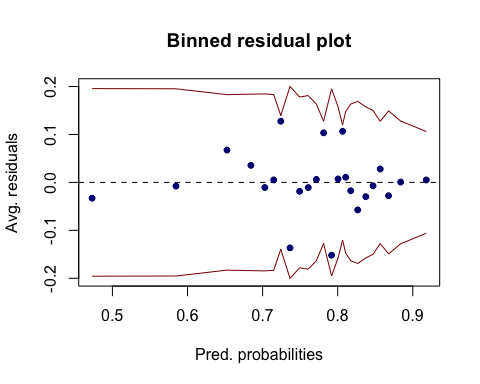
\includegraphics{revised_part1_code092721_files/figure-latex/unnamed-chunk-4-1.pdf}

\includegraphics{revised_part1_code092721_files/figure-latex/unnamed-chunk-5-1.pdf}

\includegraphics{revised_part1_code092721_files/figure-latex/unnamed-chunk-6-1.pdf}

\includegraphics{revised_part1_code092721_files/figure-latex/unnamed-chunk-7-1.pdf}

\includegraphics{revised_part1_code092721_files/figure-latex/unnamed-chunk-8-1.pdf}

\includegraphics{revised_part1_code092721_files/figure-latex/unnamed-chunk-9-1.pdf}

\includegraphics{revised_part1_code092721_files/figure-latex/unnamed-chunk-10-1.pdf}

\includegraphics{revised_part1_code092721_files/figure-latex/unnamed-chunk-11-1.pdf}

\includegraphics{revised_part1_code092721_files/figure-latex/unnamed-chunk-12-1.pdf}

\begin{verbatim}
## `geom_smooth()` using formula 'y ~ x'
\end{verbatim}

\includegraphics{revised_part1_code092721_files/figure-latex/unnamed-chunk-13-1.pdf}
It appears that we lack data for higher values of earnings for
participants who did not drop out of high school, and lower values of
earnings for participants who dropped out of high school. Thus, we will
not consider this interaction in our baseline model.

\hypertarget{model}{%
\subsection{Model}\label{model}}

\hypertarget{selection-of-baseline-model}{%
\subsubsection{Selection of Baseline
Model}\label{selection-of-baseline-model}}

\begin{verbatim}
## 
## Call:
## lm(formula = growth ~ treat + age + married + educ + race + nodegree, 
##     data = policy)
## 
## Residuals:
##      Min       1Q   Median       3Q      Max 
## -29495.5  -4045.3   -807.8   3883.0  30097.9 
## 
## Coefficients:
##             Estimate Std. Error t value Pr(>|t|)   
## (Intercept)  3566.46    2614.85   1.364  0.17310   
## treat1       2168.00     839.36   2.583  0.01003 * 
## age           -91.56      33.95  -2.697  0.00719 **
## married1    -1806.05     702.71  -2.570  0.01040 * 
## educ          101.82     170.06   0.599  0.54958   
## race2        -584.68     825.80  -0.708  0.47921   
## race3         690.48    1012.10   0.682  0.49536   
## nodegree1     451.15     913.09   0.494  0.62142   
## ---
## Signif. codes:  0 '***' 0.001 '**' 0.01 '*' 0.05 '.' 0.1 ' ' 1
## 
## Residual standard error: 7487 on 605 degrees of freedom
## Multiple R-squared:  0.0628, Adjusted R-squared:  0.05196 
## F-statistic: 5.791 on 7 and 605 DF,  p-value: 1.639e-06
\end{verbatim}

\hypertarget{model-assessment-of-baseline-model}{%
\subsubsection{Model Assessment of Baseline
Model}\label{model-assessment-of-baseline-model}}

\emph{Assessment of Linearity}

\includegraphics{revised_part1_code092721_files/figure-latex/unnamed-chunk-15-1.pdf}

\includegraphics{revised_part1_code092721_files/figure-latex/unnamed-chunk-16-1.pdf}

\emph{Assessment of Independence and Equal Variance in the Error Term}

We evaluated the assumptions of independence and equal variance in the
error by checking the plot of residuals versus fitted values

\includegraphics{revised_part1_code092721_files/figure-latex/unnamed-chunk-17-1.pdf}

\emph{Assessment of Normality in the Error Term}

\includegraphics{revised_part1_code092721_files/figure-latex/unnamed-chunk-18-1.pdf}

\emph{Assessment of Outliers}

\includegraphics{revised_part1_code092721_files/figure-latex/unnamed-chunk-19-1.pdf}

\emph{Model Selection}

Forward Model Selection with AIC

\begin{verbatim}
## 
## Call:
## lm(formula = growth ~ treat + re75 + age_c + treat:age_c, data = policy)
## 
## Residuals:
##      Min       1Q   Median       3Q      Max 
## -27082.2  -4108.9   -762.4   4087.5  29409.5 
## 
## Coefficients:
##                Estimate Std. Error t value Pr(>|t|)    
## (Intercept)  2470.15639  419.43367   5.889 6.42e-09 ***
## treat1       2254.80610  662.77365   3.402 0.000713 ***
## re75           -0.40766    0.09154  -4.454 1.01e-05 ***
## age_c        -149.51500   33.16067  -4.509 7.82e-06 ***
## treat1:age_c  246.33876   82.53334   2.985 0.002952 ** 
## ---
## Signif. codes:  0 '***' 0.001 '**' 0.01 '*' 0.05 '.' 0.1 ' ' 1
## 
## Residual standard error: 7343 on 608 degrees of freedom
## Multiple R-squared:  0.09389,    Adjusted R-squared:  0.08792 
## F-statistic: 15.75 on 4 and 608 DF,  p-value: 2.844e-12
\end{verbatim}

\emph{Assessment of Linearity}

\includegraphics{revised_part1_code092721_files/figure-latex/unnamed-chunk-21-1.pdf}

\includegraphics{revised_part1_code092721_files/figure-latex/unnamed-chunk-22-1.pdf}

\emph{Assessment of Independence and Equal Variance in the Error Term}

We evaluated the assumptions of independence and equal variance in the
error by checking the plot of residuals versus fitted values

\includegraphics{revised_part1_code092721_files/figure-latex/unnamed-chunk-23-1.pdf}

\emph{Normality}

\includegraphics{revised_part1_code092721_files/figure-latex/unnamed-chunk-24-1.pdf}

We carried out several iterations of transformations of the variables to
improve the condition of normality in the error term but no noticeable
improvement was found. Since the points do not sharply deviate from the
45 degree line, our model does not violate the normality assumption.

\emph{Assessment of Outliers}

\includegraphics{revised_part1_code092721_files/figure-latex/unnamed-chunk-25-1.pdf}

There are no outliers with high leverage and influential points.

\emph{Assessment of Multicollinearity}

\begin{verbatim}
  treat1         re75        age_c treat1:age_c 
1.048967     1.034400     1.220503     1.228833 
\end{verbatim}

The highest Variance Inflation Factor (VIF) was 1.23, which is
substantially less than the threshold for concern.

\hypertarget{final-model-results}{%
\subsubsection{Final Model Results}\label{final-model-results}}

Below is a summary of our final model

Call: lm(formula = growth \textasciitilde{} treat + re75 + age\_c +
treat:age\_c, data = policy)

Residuals: Min 1Q Median 3Q Max -27082.2 -4108.9 -762.4 4087.5 29409.5

Coefficients: Estimate Std. Error t value
Pr(\textgreater\textbar t\textbar)\\
(Intercept) 2470.15639 419.43367 5.889 6.42e-09 \textbf{\emph{ treat1
2254.80610 662.77365 3.402 0.000713 }} re75 -0.40766 0.09154 -4.454
1.01e-05 \textbf{\emph{ age\_c -149.51500 33.16067 -4.509 7.82e-06 }}
treat1:age\_c 246.33876 82.53334 2.985 0.002952 ** --- Signif. codes: 0
`\emph{\textbf{' 0.001 '}' 0.01 '}' 0.05 `.' 0.1 ' ' 1

Residual standard error: 7343 on 608 degrees of freedom Multiple
R-squared: 0.09389, Adjusted R-squared: 0.08792 F-statistic: 15.75 on 4
and 608 DF, p-value: 2.844e-12

The mathematical equation of the final model is:

\$y\_\{i\}(re78- re74) = \beta \emph{\{0\} + \beta }\{1\}x\_\{i1\}(age)+
\beta \emph{\{2\}x}\{i2\}(married)+
\beta \emph{\{3j\}x}\{i3\}(treat)+\textbackslash{}\beta \emph{\{4j\}x}\{i1\}x\_\{i3\}(treat:age)+\beta \emph{\{5j\}x}\{i1\}x\_\{i2\}(married:age)+
\epsilon \$

All the predictor variables in the final model have a significant effect
on real annual earnings. These predictor variables are the training
status (`treat'), real annual earnings in 1975 (`re75), age ('age\_c')
and the interaction between training status and age (`treat1:age\_c').

Question 1:

There is statistically significant evidence that training has positive
relationship with the growth of income from 1974 to 1978, accounting for
other effects and interaction between job training and age. The
difference in real annual earnings from 1974 to 1978 increases by
\$2,254.80 for participants who were trained compared to participants
who were not trained, keeping all other predictor variables constant.

Question 2:

After computing``two-sided'' confidence intervals for the effect of
training.

\begin{verbatim}
                2.5 %       97.5 %
\end{verbatim}

(Intercept) 1646.4417604 3293.8710190 treat1 953.2025673 3556.4096418
re75 -0.5874204 -0.2278939 age\_c -214.6383594 -84.3916349 treat1:age\_c
84.2537263 408.4237942

Accounting for all other predictors, we are 95\% confident that the
difference in real annual earnings from 1974 to 1978 increases by an
amount between \$953.20 and \$3,556.41 for participants who were trained
compared to participants who were not trained.

Question 3:

\begin{verbatim}
## Analysis of Variance Table
## 
## Model 1: growth ~ treat + re75 + age_c + treat:age_c
## Model 2: growth ~ treat + re75 + age_c + treat:age_c + treat:race
##   Res.Df        RSS Df Sum of Sq      F Pr(>F)
## 1    608 3.2786e+10                           
## 2    604 3.2596e+10  4 189428682 0.8775  0.477
\end{verbatim}

After carrying out an F-test to determine if the effect of training on
earnings differs by demographic groups, we had a p-value of 0.447. This
means there is no statistically significant evidence that the effect of
training on earnings differs by demographic groups.

Question 4:

Apart from the training status of participants, the age, real annual
earnings in 1975 and interactions between training status and age have a
significant effect on the growth in real annual earnings from 1974 to
1978. The predictor variable that had the most effect on the growth in
real annual earnings is the age of participants. Keeping all other
predictor variables constant, the growth in real annual earnings
decreased by \$149.52 for every year older that a participant gets.
Also, keeping all other predictor variables constant, the growth in real
annual earnings decreased by \$0.41 for every dollar increase in real
annual earnings for 1975.

\end{document}
